\section{Aula 4}
\label{sec:4}

\subsection{Sistemas Elétricos}
Operar o sistema é definir, a cada etapa do tempo, quais usinas serão acionadas para suprir a demanda de energia elétrica. Além disso os
recursos disponíveis ,por exemplo usinas, possuem capacidades $(G_{i})$ diferentes
e, sobretudo, custos de operação distintos $(c_{i})$. O critério é atender uma demanda $d$ ao menor custo operativo possível garantindo confiabilidade. 

\textbf{Exemplo}

Dois geradores apresentam ofertas de preço e quantidade de geração$(c_{i},G_{i})$ e precisam atender a demanda dos consumidores, que
totaliza $(d)$. No qual o primeiro gerador tem capacidade máxima de produção de $100$ MW e o custo de $100$R\$/MWh enquanto o segundo gerador tem
capacidade máxima de produção de $50$ MW e o custo de $150$R\$/MWh. Esses geradores precisam atender uma demanda de $120$MW (Figura \ref{fig:aula4-1}). Por conveniência, será trabalhado num horizonte de tempo de uma hora, para que potencia
e energia sejam a mesma coisa. e assumindo que a potencia é constante.
\begin{figure}[H]
\begin{centering}
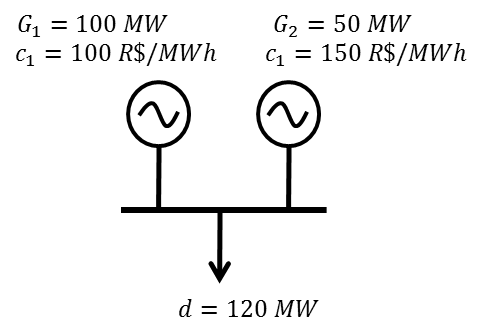
\includegraphics{aula4-1}\protect\caption{\label{fig:aula4-1} Exemplo }
\end{centering}
\end{figure}
Para atender a demanda com esses dois geradores uma possível solução para o problema seria utilizar a potencia do mais barato e depois se necessário utilizar a do mais caro. Essa solução é conhecida como ordem de mérito em custo. Então será necessário utilizar os $100$MW
do primeiro gerador e completar com $20$MW do segundo gerador para assim, atender a demanda (Figura \ref{fig:aula4-2}).
\begin{figure}[H]
\begin{centering}
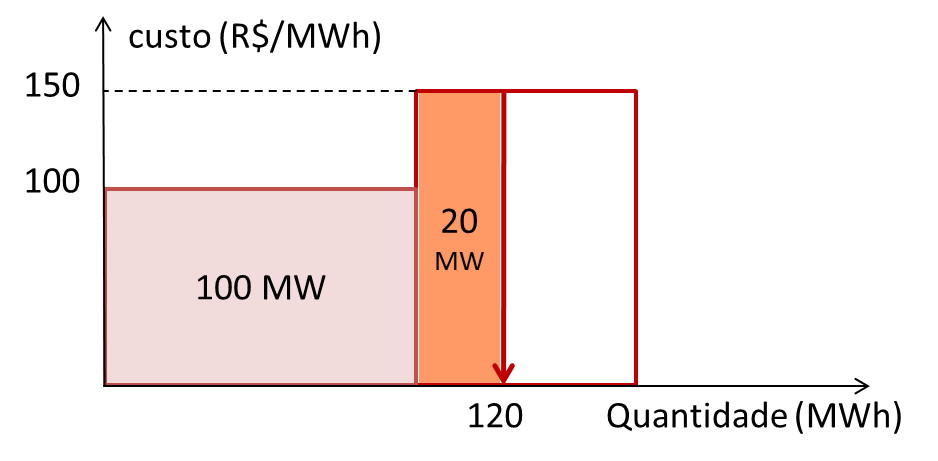
\includegraphics[scale=0.7]{aula4-2}\protect\caption{\label{fig:aula4-2} Despacho por ordem de custo }
\end{centering}
\end{figure}
A modelagem do problema será dado por:
\begin{align}
    & \underset{g\geq0}{\text{Min}} \hspace{1cm} 100g_1+150g_2 \label{eq1} \\
    & \text{s.a}  \hspace{2.2cm} g_1+g_2 \geq 120; \label{eq2} \\
    &             \hspace{2.65cm} g_1\leq 100, \label{eq3}\\
    &             \hspace{2.65cm} g_2\leq 50. \label{eq4}
\end{align}

Assim, a visualização gráfica com a área viável é apresentado na figura \ref{fig:aula4-3}.
\begin{figure}[H]
\begin{centering}
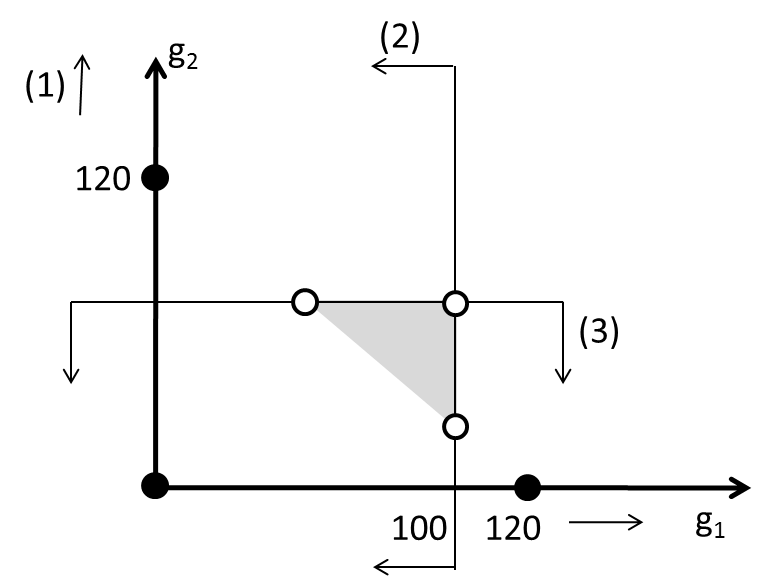
\includegraphics[scale=0.7]{aula4-3}\protect\caption{\label{fig:aula4-3} Gráfico exemplo }
\end{centering}
\end{figure}
Adicionando o gradiente e verificando a solução ótima do problema:

\begin{figure}[H]
\begin{centering}
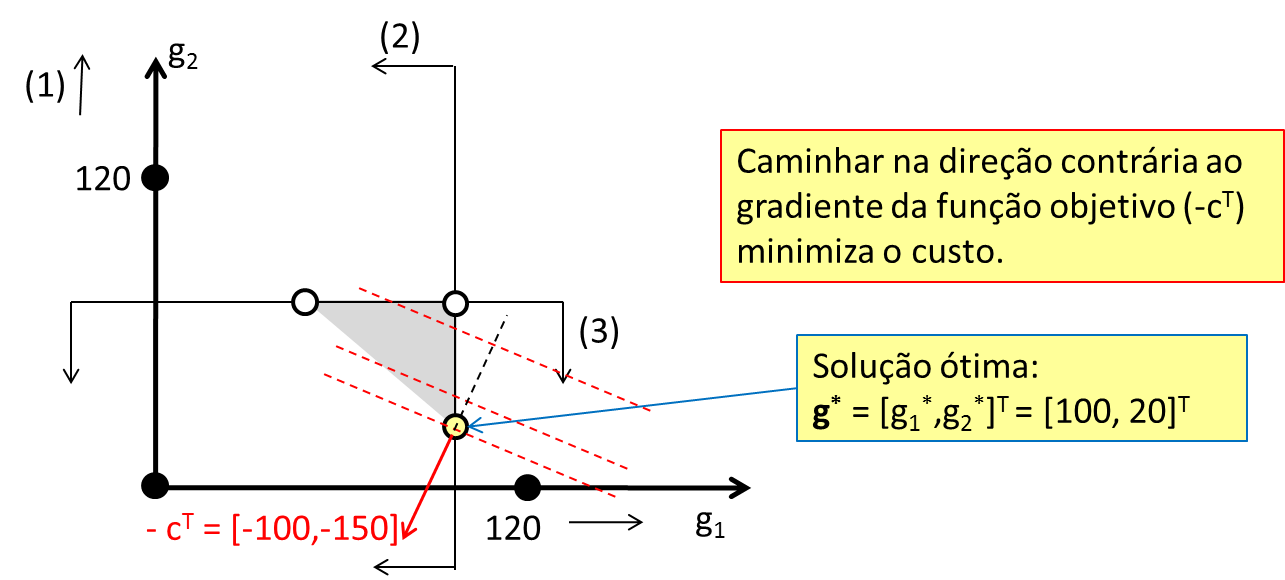
\includegraphics[scale=0.70]{aula4-4}\protect\caption{\label{fig:aula4-4} Gráfico exemplo gradiente }
\end{centering}
\end{figure}

\begin{figure}[H]
\begin{centering}
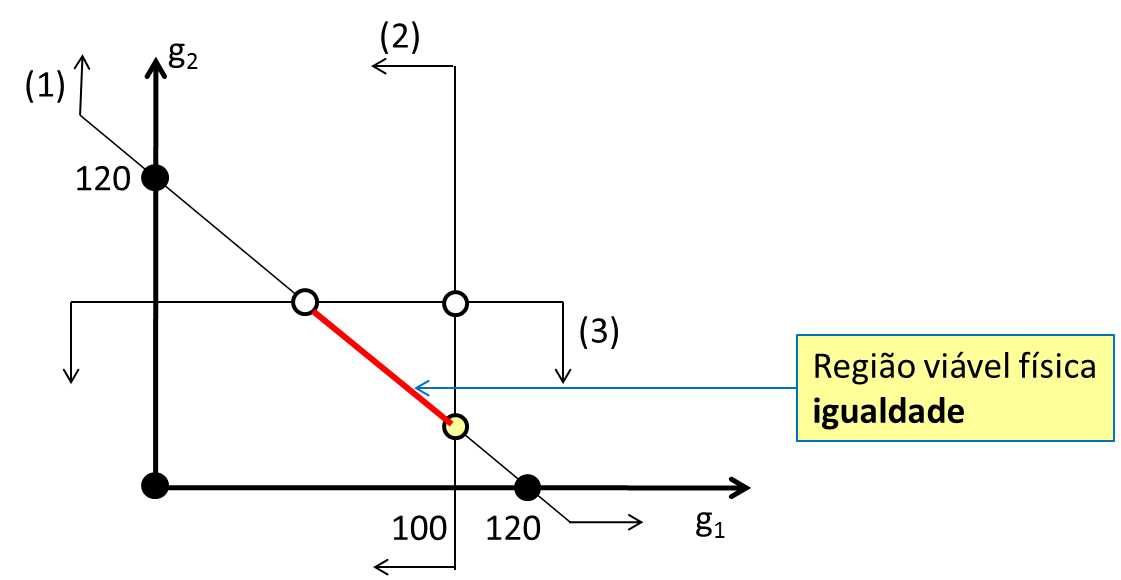
\includegraphics[scale=0.8]{aula4-5}\protect\caption{\label{fig:aula4-5} Gráfico exemplo igualdade}
\end{centering}
\end{figure}

Através da figura (\ref{fig:aula4-5}), é possível concluir que a restrição (\ref{eq2}) será alterada, conforme apresentado:
\begin{align}
    & \underset{g\geq0}{\text{Min}} \hspace{1cm} 100g_1+150g_2 \label{eq5} \\
    & \text{s.a}  \hspace{2.2cm} g_1+g_2 = 120; \label{eq6} \\
    &             \hspace{2.65cm} g_1\leq 100, \label{eq7}\\
    &             \hspace{2.65cm} g_2\leq 50. \label{eq8}
\end{align}
A primeira restrição(\ref{eq6}) é o objetivo primário por ser necessário atender a demanda independente do custo gerado, e posteriormente será avaliado o menor custo de geração. Se por exemplo o nosso objetivo primário fosse atender o custo, a melhor solução para o problema é não produzir. Assim,primeiramente precisamos  atender as restrições para depois avaliar o objetivo, no caso menor custo.
Então o problema de despacho pode ser modelado da seguinte maneira,
\begin{align}
    & \underset{g\geq0}{\text{Min}} \hspace{1cm} \sum_{i=1}^{n}c_{i}\cdot g_{i} \label{eq9} \\
    & \text{s.a}  \hspace{2.2cm} \sum_{i=1}^{n}g_{i}\geq d; \label{eq10} \\
    &             \hspace{2.65cm}g_{i}\leq G_{i} \forall i=1,...,n. \label{eq11}
\end{align}

O objetivo é minimiza a soma dos custos variáveis referente a sua geração (equação \ref{eq9}) , sendo que precisamos atender a demanda (equação \ref{eq10}) e atendendo o máximo de geração de cada usina (equação \ref{eq11}).
Supondo que a demanda precise de um MWH a mais do problema modelado anteriormente,qual o custo desse MWH a ser atendido?
O objetivo descobrir o custo adicional do próximo MWH é interessante
para saber quanto cobrar a mais no caso de entrar uma MWH no modelo.
O conceito de usina marginal ou unidade marginal é a usina que está na
margem das usinas que estão produzindo, ou seja, o ultimo gerador
produzindo.Assim, é formado o custo marginal do sistema.

O custo pode ser representado por,
\[
\Delta C^{*}(d)=C^{*}(d+1)-C^{*}(d).
\]

Temos que,

\[
\frac{\partial C^{*}(d)}{\partial d}=\lim_{\Delta\rightarrow0^{+}}\frac{C^{*}(d+\Delta-C^{*}(d))}{\Delta} ,
\]


\[
\frac{\partial C^{*}(d)}{\partial d}=c_{i^{*}},
\]
$i^{*}$é o gerador marginal.
Como no exemplo apenas o gerador 2 possui potencia para atender o
próximo MWH, então seu custo adicional será o custo $c_{2}$ ,\[
\Delta C^{*}(d)=[C^{*}(d)+c_{2}\cdot1]-C^{*}(d)=c_{2},
\]
 e pode ser representado na figura abaixo:

\begin{figure}[H]
\begin{centering}
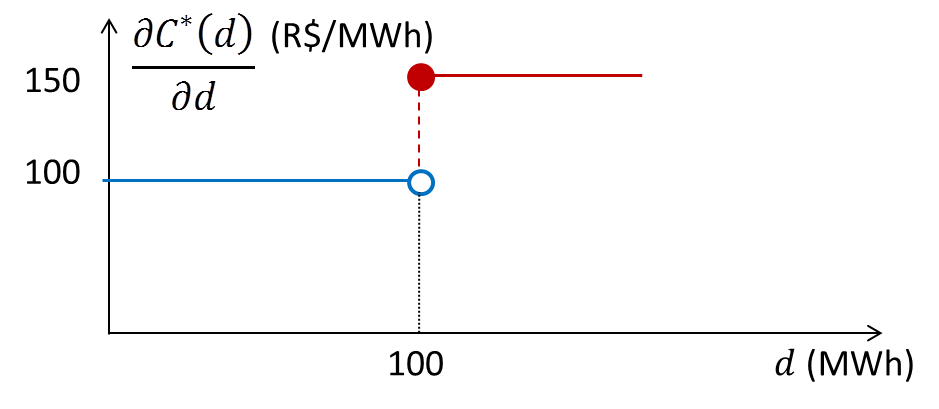
\includegraphics[scale=0.8]{aula4-6}\protect\caption{\label{fig:aula4-6} Derivada nos pontos}
\end{centering}
\end{figure}
Então aplicado ao exemplo anterior será dado por:
\begin{figure}[H]
\begin{centering}
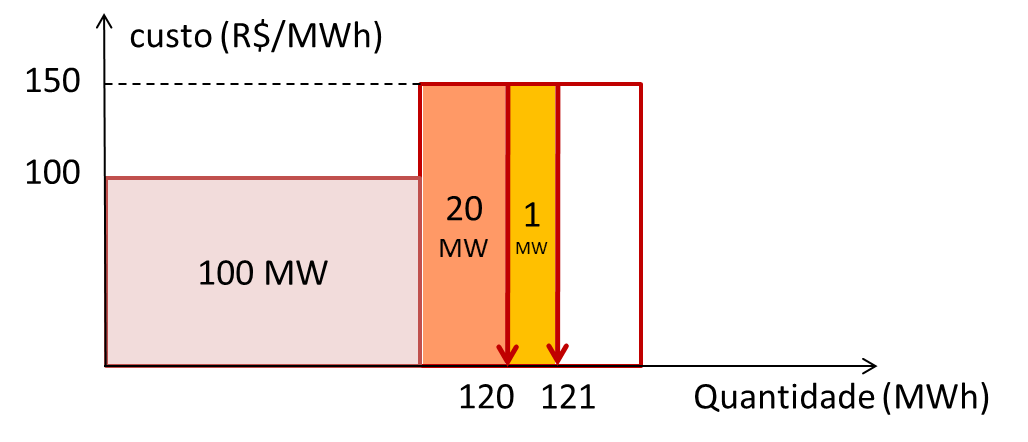
\includegraphics[scale=0.8]{aula4-7}\protect\caption{\label{fig:aula4-7} Gráfico exemplo com custo adicional}
\end{centering}
\end{figure}
A função custo será dada pela figura (\ref{fig:aula4-8}) e possui propriedades importantes:
\begin{enumerate}
\item é linear por partes;
\item tem primeira derivada descontínua;
\item é crescente;
\item é convexa;
\end{enumerate}
\begin{figure}[H]
\begin{centering}
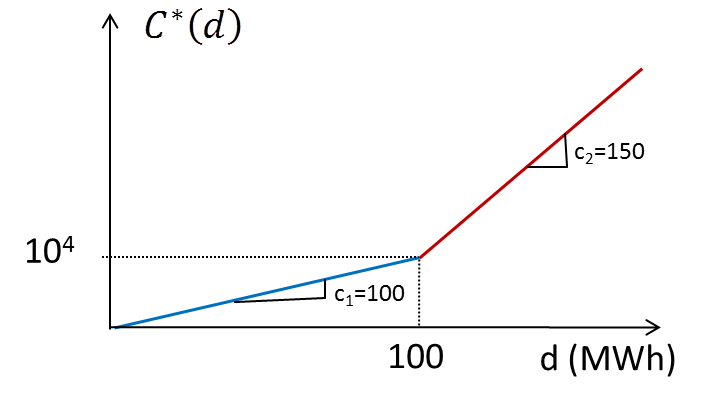
\includegraphics[scale=0.8]{aula4-8}\protect\caption{\label{fig:aula4-8} Função custo}
\end{centering}
\end{figure}
\subsection{Teoria da dualidade}
\begin{enumerate}
\begin{itemize}
\item Como funciona o processo de “dualização” de restrições (relaxação langrangeana)?
\begin{equation*}
\begin{aligned}
& z_{p}^{*}=\underset{x\geq0}{\text{Max}}
& & c^{T}x \\
& \text{s.a}
& & Ax \leq b.
\end{aligned}
\end{equation*}
\item O processo de ``dualização'' implica em relaxar alguma das restrições
(ou todas) do problema prima e incorporar uma penalização na função
objetivo sobre a viabilidade das soluções.
\begin{equation*}
\begin{aligned}
& z_{p}^{*}\leq \theta(y)=\underset{x\geq0}{\text{Max}}
& & c^{T}x+y^{T}(b-Ax)  \forall  y\geq 0 \\
& \text{s.a}
& & Ax \leq b.
\end{aligned}
\end{equation*}
\[
z_{p}^{*}\leq\theta(y)\leq\phi(y)=\max_{x\geq0}c^{T}\cdot x+y^{T}\cdot(b-A\cdot x)\forall y\geq0
\]
Uma interpretação para a variável dual($y^{T}(b-A\cdot x)$) no exemplo dado na aula 1: O dono da fábrica agora pode vender ou comprar a sobra ou déficit de insumos em “um mercado” (ilimitado) por preço y.
\item Como se comporta a função dual lagrangeana?

\[
z_{p}^{*}\leq\phi(y)=\max_{x\geq0}c^{T}\cdot x+y^{T}\cdot(b-A\cdot x)\forall y\geq0
\]
\item Dado um vetor $y$ de multiplicadores de Lagrange,
\[
z\leq\phi(y)=\max_{x\geq0}(c^{T}-y^{T}\cdot A)\cdot x+y^{T}\cdot b=\left\{ \begin{array}{c}
y^{T}\cdot b,sec^{T}-y^{T}\cdot A\leq0\\
+\infty,casocontr\acute{a}rio
\end{array}\right\} 
\]
\item O processo de relação lagrangeana busca uma vetor y que minimize $\phi(y)$. Logo, o segundo caso (que proporciona valor infinito) será sempre evitado.A interpretação para esse comportamento é:
\item[-] Se o lucro unitário de produção $(c^{T})$ for inferior à receita de venda de seus insumos $(y^{T}A)$ no mercado ao preço $y$ , então paramos a produção e vendemos todos os insumos no mercado, resultando em um lucro de $y^{T}b$.
\item[-] Caso contrário, ocorre a possibilidade de arbitragem, onde podemos comprar no mercado os insumos por preços que geram um custo inferior ao lucro de produção. Assim, compramos infinito e vendemos infinito, obtendo assim resultado ilimitado.
\item O problema dual busca um vetor y que minimize $\phi(y)$.Logo, o segundo caso será sempre evitado.
$$
z\leq\min_{y\geq0}\phi(y)=\min_{y\geq0}\left\{ \begin{array}{c}
y^{T}\cdot b,sec^{T}-y^{T}\cdot A\leq0\\
+\infty,casocontr\acute{a}rio
\end{array}\right\} =\begin{array}{cc}
\min_{y\geq0} & y^{T}\cdot b\\
s.a: & y^{T}\cdot A\geq c^{T}
\end{array}
$$
Assim, Quais são os preços y's que minimizam essa função. A busca pelos preços de mercado que deixa o produtor indiferente entre produzir e vender os insumos nos mercados.
\item Assim, temos o seguinte par primal-dual:
$$
z_{p}^{*}=\begin{array}{cc}
\max_{x\geq0} & c^{T}\cdot x\\
s.a: & A\cdot x\leq b
\end{array}\leq z_{d}^{*}=\begin{array}{cc}
\min_{y\geq0} & y^{T}\cdot b\\
s.a: & y^{T}\cdot A\geq c^{T}
\end{array}
$$
\item O teorema da dualidade fraca diz que (Primal de Maximização):
\item[-]  O valor mínimo do problema Dual ( de minimização) é superior ao máximo do problema primal (maximização).
\item[-] Isso torna-se óbvio depois de mostrado o processo de construção do
dual da maneira que apresentamos aqui. Este foi concebido para sempre
gerar um limite superior para o problema primal.
\item O teorema da dualidade Forte diz que ( Primal de Maximização):
\item[-] No ótimo o valor da função objetivo de qualquer par primal-dual decorrente de um problema de programação linear é sempre o mesmo!
$$
z_{p}^{*}=\begin{array}{cc}
\max_{x\geq0} & c^{T}\cdot x\\
s.a: & A\cdot x\leq b
\end{array} = z_{d}^{*}=\begin{array}{cc}
\min_{y\geq0} & y^{T}\cdot b\\
s.a: & y^{T}\cdot A\geq c^{T}
\end{array}
$$
\begin{figure}[H]
\begin{centering}
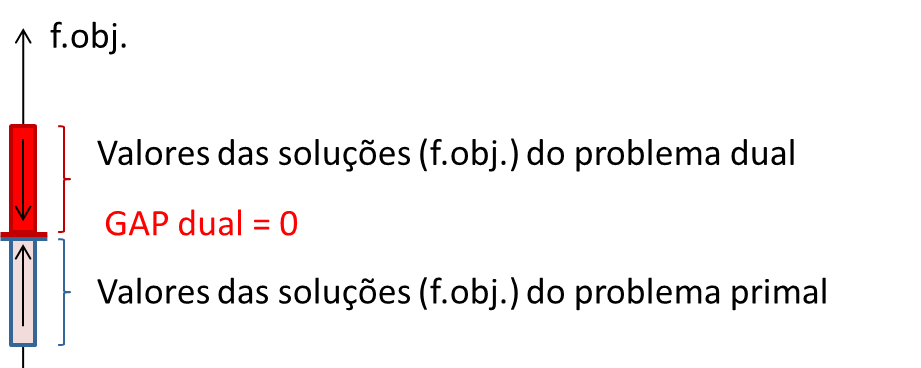
\includegraphics[scale=0.8]{aula4-9}\protect\caption{\label{fig:aula4-9} GAP dual}
\end{centering}
\end{figure}
\item Talvez a mais importante, ou pelo menos mais conhecida e difundida
em diversas áreas, devido à relação entre o problema primal e o dual
seja a interpretação da variável dual como ``preço sombra'' ou custo
marginal dos recursos:
\item[-] Em problemas convexos, em que vale a dualidade forte, a variável dual pode ser interpretada como a derivada parcial do valor ótimo da função
objetivo do primal, com relação ao lado direito da restrição associada
a esta variável.
\item[-] Que em ultima análise é o multiplicador de lagrange
\[
z_{p}^{*}=z_{d}^{*}=y^{*T}\cdot b
\]


\[
\frac{\partial z_{p}^{*}}{\partial b}=\left[\frac{\partial z_{p}^{*}}{\partial b_{1}},...,\frac{\partial z_{p}^{*}}{\partial b_{m}}\right]=\left[y_{1}^{*},...,y_{m}^{*}\right]=y^{*T}.
\]

\end{itemize}
\end{enumerate}
\textbf{Exemplo: despacho centralizado vs. competição perfeita}

O despacho ótimo ``centralizado'' de um período, que visa atender
uma demanda $d$ (MWh) utilizando os recursos disponíveis (capacidade
$G_{i}$) é dado pelo seguinte problema:
\begin{align}
    & \underset{g\geq0}{\text{Min}} \hspace{1cm} \sum_{i=1}^{n}c_{i}\cdot g_{i} \label{eq12} \\
    & \text{s.a}  \hspace{2.2cm} \sum_{i=1}^{n}g_{i}\geq d; \label{eq13} \\
    &             \hspace{2.65cm}g_{i}\leq G_{i} \forall i=1,...,n. \label{eq14}
\end{align}

Para que este problema atinja o seu objetivo, é importante que os
agentes informe os seus reais custo operativos e capacidades ($c_{i},G_{i}$).
Um processo iterativo (competição) que controla o preço de mercado
da energia, onde os geradores (price-takers) ofertam preço (custos reais) e quantidade (capacidades máximas), visando maximizar os seus lucros individualmente com a venda de energia através de um leilão de preço uniforme, proporciona o mesmo despacho (solução de geração) que o despacho de
mínimo custo.
Assim, começamos por dualização a restrição de atendimento à demanda. Onde, para todo $\pi\geq0$ teremos a seguinte relação:
\[
C^{*}\geq C_{d}^{*}(\pi)=Min_{g\geq0}\sum_{i=1}^{n}c_{i}\cdot g_{i}+\pi\cdot\left(d-\sum_{i=1}^{n}g_{i}\right)
\]

\[
s.a \, g_{i}\leq G_{i}\forall i=1, ... ,n.
\]
Em seguida, rearranjamos os termos de maneira a colocar o $g_{i}$ em evidência:


\[
C^{*}\geq C_{d}^{*}(\pi)=Min_{g\geq0}\pi\cdot d-\sum_{i=1}^{n}(\pi-c_{i})\cdot g_{i}
\]


\[
s.a \, g_{i}\leq G_{i}\forall i=1,...,n.
\]


Como o primeiro termo não depende da decisão $g$, este pode ser colocado fora do  $min$ e podemos verificar que o $min$ de uma função negativa é o $max$ desta função colocando o sinal de negativo para fora da função $max$. Temos que ,
\[
C^{*}\geq C_{d}^{*}(\pi)=\pi\cdot d-\sum_{i=1}^{n}Max_{g\geq0_{i}}(\pi-c_{i})\cdot g_{i}
\]


\[
s.a \, g_{i}\leq G_{i}\forall i=1,...,n.
\]
Por fim, repare que o problema de minimização pode ser decomposto
em $n$ problemas, em que cada um pode ser substituído por um de maximização.

Assim, dado o preço do mercado $\pi$ é encontrado o problema de maximização da receita líquida de venda ($Max_{g\geq0_{i}}(\pi-c_{i})\cdot g_{i}$).
O problema resultante é o problema em que cada agente gerador visa maximizar a sua renda vendendo energia a um preço $\pi$(R\$/MWh) e a demanda (inelástica) paga o mesmo preço pela aquisição dessa energia.
Onde,
\[
C^{*}\geq Max_{\pi\geq0}\pi\cdot d-\sum_{i=1}^{n}R_{i}^{*}(\pi)
\]


\[
R_{i}^{*}(\pi)=Max_{g_{i}\geq0}(\pi-c_{i})\cdot g_{i}
\]


\[
s.a \, g_{i}\leq G_{i}\forall i=1,...,n.
\]

\begin{figure}[H]
\begin{centering}
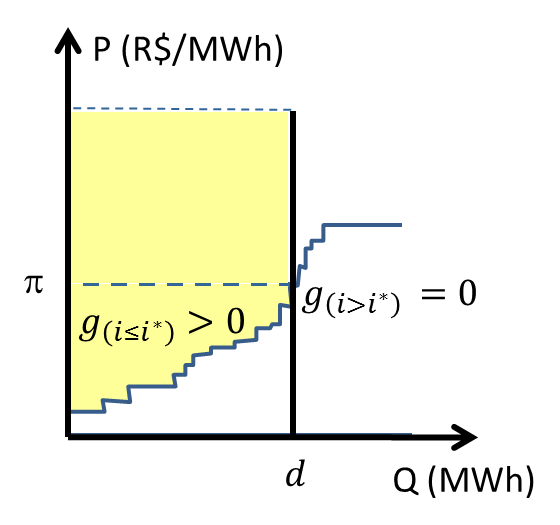
\includegraphics[scale=0.8]{aula4-10}\protect\caption{\label{fig:aula4-10} Operação centralizada vs competitiva}
\end{centering}
\end{figure}
E se a capacidade de geração não for suficiente para suprir a demanda?
\begin{figure}[H]
\begin{centering}
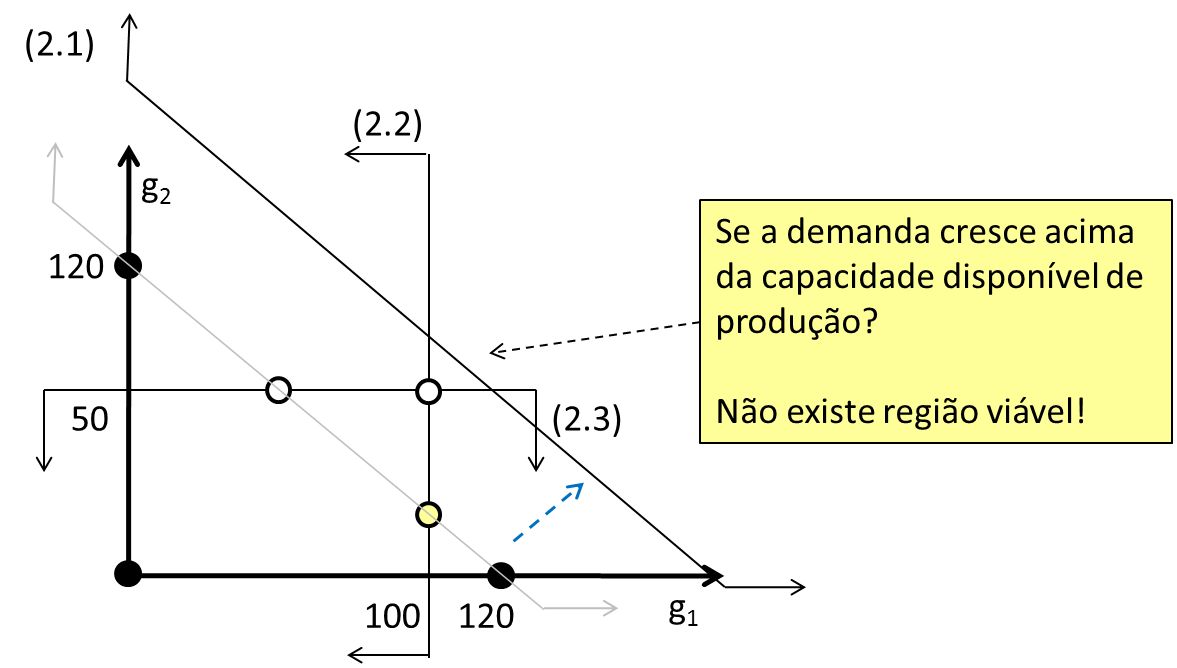
\includegraphics[scale=0.5]{aula4-11}\protect\caption{\label{fig:aula4-11} Gráfico com o aumento da demanda}
\end{centering}
\end{figure}
Corte de carga (déficit)

Se a demanda for maior que a soma das capacidades máximas, então o
problema é inviável. Porém,na prática o problema não é inviável, mas uma fração da demanda não será suprida: ``corte de carga'' ou déficit (diferente de racionamento).Na realidade o sistema é operado cortando algumas cargas (diminuindo as cargas) por exemplo uma área da distribuidora ,desliga algum consumidor,desligamentos seletivos, etc.
\begin{figure}[H]
\begin{centering}
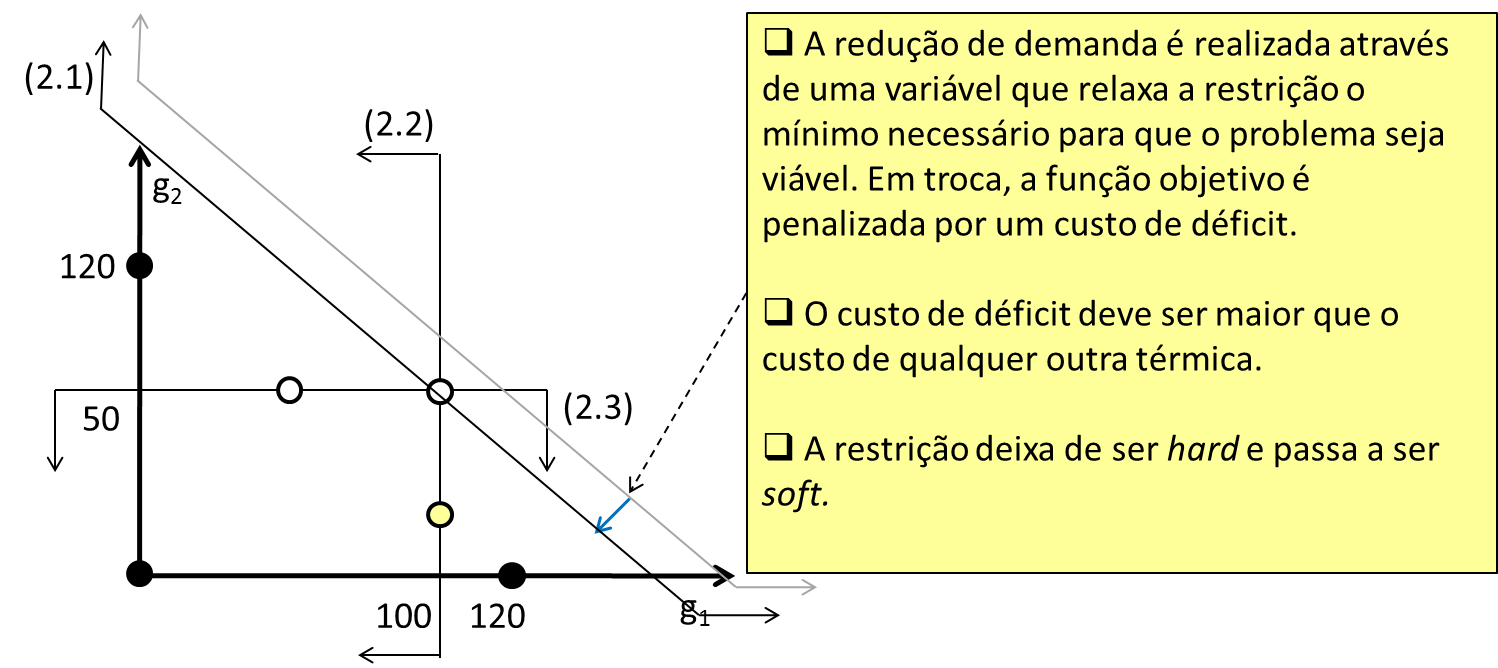
\includegraphics[scale=0.7]{aula4-12}\protect\caption{\label{fig:aula4-12} Viabilidade do proble,a }
\end{centering}
\end{figure}
Caso falte capacidade de produção, sera necessário transformar um restrição hard (inicialmente a restrição de atender à demanda) para um restrição suavizada (atender a demanda sempre que possível) então será necessário diminuir a demanda assim, esse corte de carga é ótimo. 
Para isso introduzimos uma variável ao problema que age como se
fosse um gerador, porem é um corte de carga.Essa variável adicionada ao problema  é uma variável de decisão e é penalizada no problema na função objetivo com um custo de deficit maior que o custo dos outros geradores.
Assim é possível construir a curva de déficit, com diferente patamares
que será modelado na seguinte maneira:
\begin{align}
    & \underset{g\geq0, r\geq0}{\text{Min}} \hspace{1cm} \sum_{i=1}^{n}c_{i}\cdot g_{i} + c_{d}\cdot r \label{eq15} \\
    & \text{s.a}  \hspace{2.2cm} \sum_{i=1}^{n}g_{i} + r\geq d \label{eq16} \\
    &             \hspace{2.65cm}g_{i}\leq G_{i} \forall i=1,...,n.\label{eq17}
\end{align}

Essa função é conhecida como custo de déficit. E será representada,

\begin{align}
    & \underset{g\geq0, r\geq0}{\text{Min}} \hspace{1cm} \sum_{i=1}^{n}c_{i}\cdot g_{i} + \sum_{j=1}^{m}c_{j}^{d}\cdot r_{j} \label{eq16} \\
    & \text{s.a}  \hspace{2.2cm} \sum_{i=1}^{n}g_{i} + \sum_{j=1}^{m}r_{j}\geq d \label{eq17} \\
    &             \hspace{2.65cm}g_{i}\leq G_{i} \forall i=1,...,n\label{eq18}\\
    &                \hspace{2.65cm}r_{j}\leq \bar{r}_{j} \forall j=1,...,m.\label{eq19}
\end{align}
A figura (\ref{fig:aula4-14}) representa a adição do custo de déficit no modelo.
\begin{figure}[H]
\begin{centering}
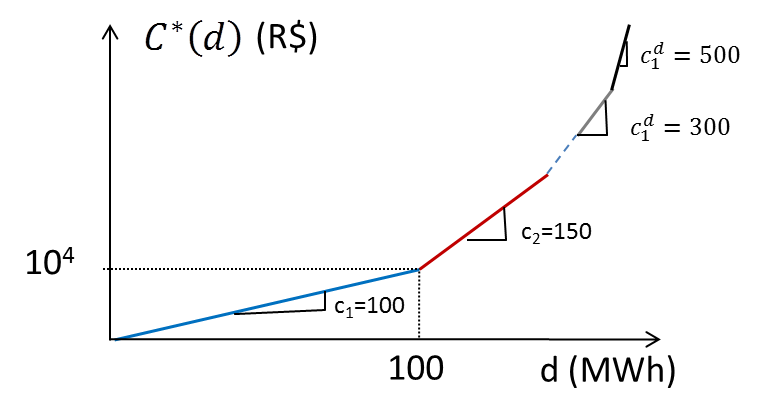
\includegraphics[scale=0.8]{aula4-14}\protect\caption{\label{fig:aula4-14} Função custo com o custo de déficit }
\end{centering}
\end{figure}

A figura (\ref{fig:aula4-15}) é conhecida como curva de duração de demanda, no eixo ($x$) está representada a frequência no ano e o eixo($y$) representa a demanda. Uma interpretação para este gráfico é que quando a demanda atingir uma carga crítica de ($5\%$) com uma duração de ($5\%$) do ano, estaríamos utilizando geradores flexíveis, geradores de base e geradores inflexível. 
Geradores de bases praticamente inflexível (exemplo:nuclear e carvão) produzem energia ($100\%$) durante o ano e possuem custo de investimento caro e custo de operação barato ou seja, são os primeiro a serem ligados.Geradores de bases flexíveis conseguem gerar e desligar se necessário com um taxa de desligamento (não acionamento), as vezes a demanda fica menor do que o custo variável destes. Geradores flexíveis  são responsáveis por atender demandas no intervalo acima, o os demais geradores são conhecidos como geradores de pico que vivem para atender aproximadamente 3\% da carga. Só em eventos raros ele será acionado para produzir. Porem,qual deve ser o valor que se paga para os geradores de pico para produzir sabendo que eles vão produzir em poucas horas.
\begin{figure}[H]
\begin{centering}
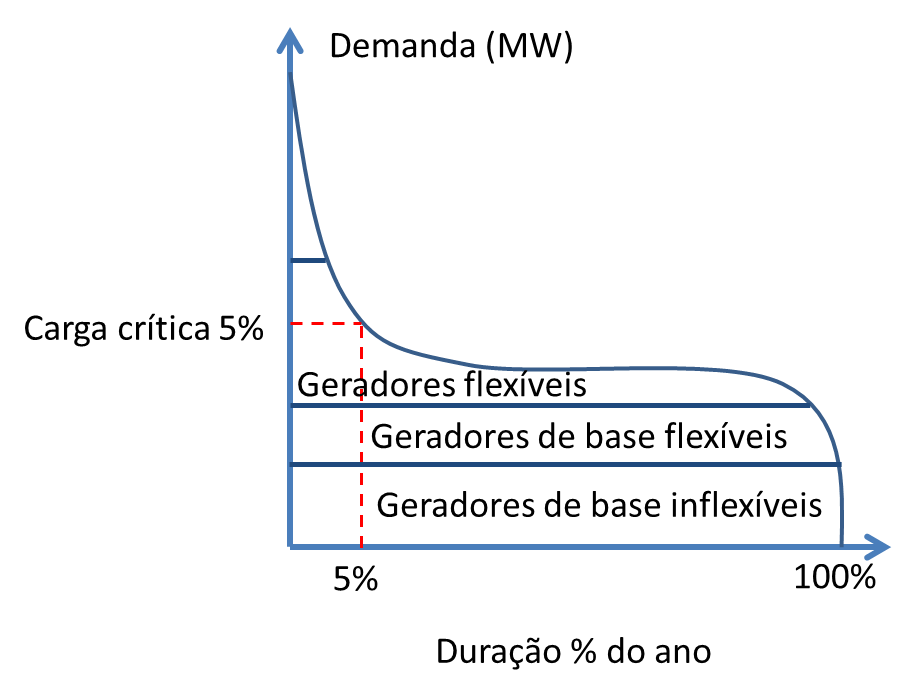
\includegraphics[scale=0.7]{aula4-15}\protect\caption{\label{fig:aula4-15}  Curva de duração de demanda}
\end{centering}
\end{figure}

\subsection{Restrições de rede}
\textbf{Exemplo}

Sejam dois geradores em locais diferentes ligados por uma linhas de transmissão onde, os geradores possuem capacidades finitas e limites de transmissão. O gerador $1$ tem capacidade máxima de produção de $100$ MW e o custo de $100$R\$/MWh enquanto o  gerador $2$  tem capacidade máxima de produção de $50$ MW e o custo de $150$R\$/MWh.Esses geradores precisam atender uma demanda de $120$MW (Figura \ref{fig:aula4-16}). O diferencial deste exemplo para o exemplo apresentando anteriormente está na linha de transmissão. O gerador $1$ pode transmitir $80$ MW e a linha de transmissão do gerador $2$ pode passar $80$MW para atender a demanda de $120$MW.
\begin{figure}[H]
\begin{centering}
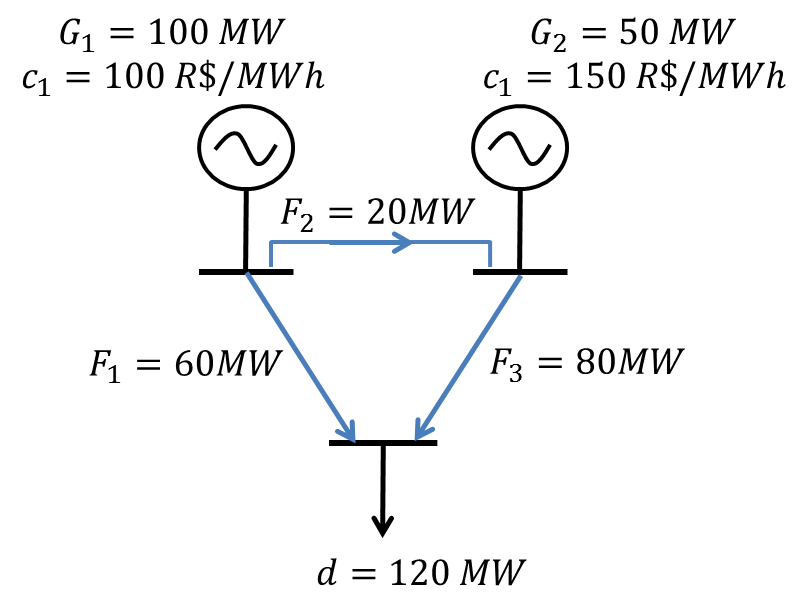
\includegraphics[scale=0.8]{aula4-16}\protect\caption{\label{fig:aula4-16} Exemplo ligado por linha de transmissão}
\end{centering}
\end{figure}
O despacho ótimo encontrado no primeiro exemplo de $g_{1}^{*}=100$ não pode ser injetado na rede, então neste caso essa solução será inviável.
A seta na (Figura \ref{fig:aula4-16}) representa o sentido do fluxo e por convenção adotaremos que quando a senta sai do gerador perde energia então temos fluxo negativo e quando entra o gerador recebe energia e assim o fluxo é positivo.

O modelo de transporte, possui esse nome por não considerar algumas características elétricas do na rede, será dado por:
\begin{itemize}
\item Restrição de atendimento à demanda (balanço de potência ou nodal)
por barra:

\[
g_{1}-f_{1}-f_{2}=0
\]


\[
g_{2}+f_{2}-f_{3}=0
\]


\[
f_{1}+f_{3}=d
\]
\item O sinal do fluxo depende da convenção: (+) se passa no sentido das setas e (-) caso contrário.
\item Então, a restrição de capacidade das linhas é:

\[
-F_{l}\leq f_{1}\leq F_{l}
\]
\item Matriz de incidência de fluxo em redes: $+1$ se a aresta $l$ chega
no vértice $i$ e $-1$ se sai:
\[
\begin{array}{ccccccc}
g_{1} &  & -f_{1} & -f_{2} &  & = & 0\\
 & g_{2} &  & +f_{2} & -f_{3} & = & 0\\
 &  & f_{1} &  & +f_{3} & = & d
\end{array}
\]
Ou seja, tudo que entra na barra é igual a tudo que sai dessa barra.
\end{itemize}
Assim, podemos montar o modelo de transporte completo do exemplo dado por:
\[
\min_{g_{i}\geq0,f_{l}}100g_{1}+150g_{2}
\]
\[
\begin{array}{ccccccc}
s.a:\\
g_{1} &  & -f_{1} & -f_{2} &  & = & 0\\
 & g_{2} &  & +f_{2} & -f_{3} & = & 0\\
 &  & f_{1} &  & +f_{3} & = & d\\
-60 & \leq & f_{1} &  &  & \leq & 60\\
-20 & \leq &  & f_{2} &  & \leq & 20\\
-80 & \leq &  &  & f_{3} & \leq & 80\\
g_{1} &  &  &  &  & \leq & 100\\
 & g_{2} &  &  &  & \leq & 50.
\end{array}
\]
\begin{figure}[H]
\begin{centering}
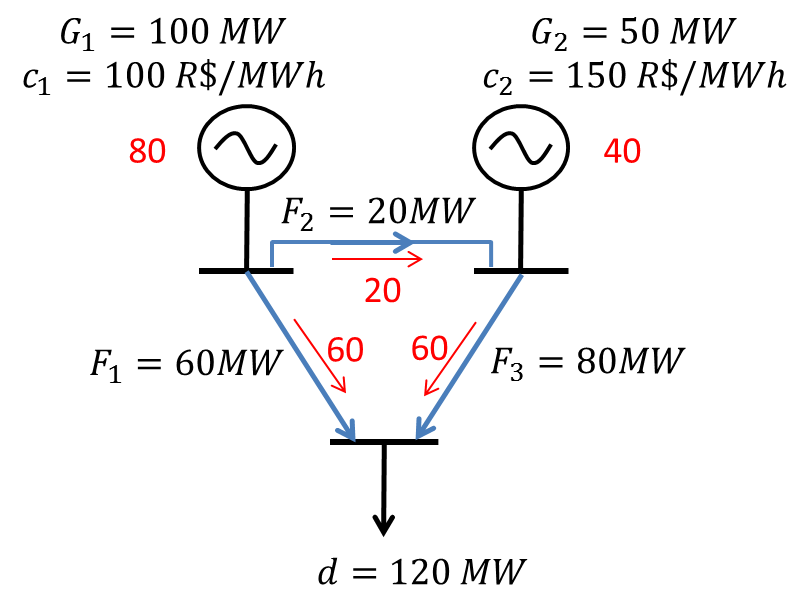
\includegraphics[scale=0.7]{aula4-17}\protect\caption{\label{fig:aula4-17} Solução ótima do exemplo}
\end{centering}
\end{figure}

A Figura (\ref{fig:aula4-17} ) representa a solução ótima do problema.

\textbf{O custo marginal nodal}
O custo de atender $1$ MWh a mais, sendo que neste exemplo podemos adicionar esse MWh para cada barra do sistema.
No caso da barra $1$, o custo adicional de operação ótima para suprir $1$ MWh será representado na figura (\ref{fig:aula4-18} ) e  modelado da seguinte maneira:
\[
\min_{g_{i}\geq0,f_{l}}100g_{1}+150g_{2}
\]
\[
\begin{array}{ccccccc}
s.a:\\
g_{1} &  & -f_{1} & -f_{2} &  & = & +1\\
 & g_{2} &  & +f_{2} & -f_{3} & = & 0\\
 &  & f_{1} &  & +f_{3} & = & d\\
-60 & \leq & f_{1} &  &  & \leq & 60\\
-20 & \leq &  & f_{2} &  & \leq & 20\\
-80 & \leq &  &  & f_{3} & \leq & 80\\
g_{1} &  &  &  &  & \leq & 100\\
 & g_{2} &  &  &  & \leq & 50.
\end{array}
\]

\begin{figure}[H]
\begin{centering}
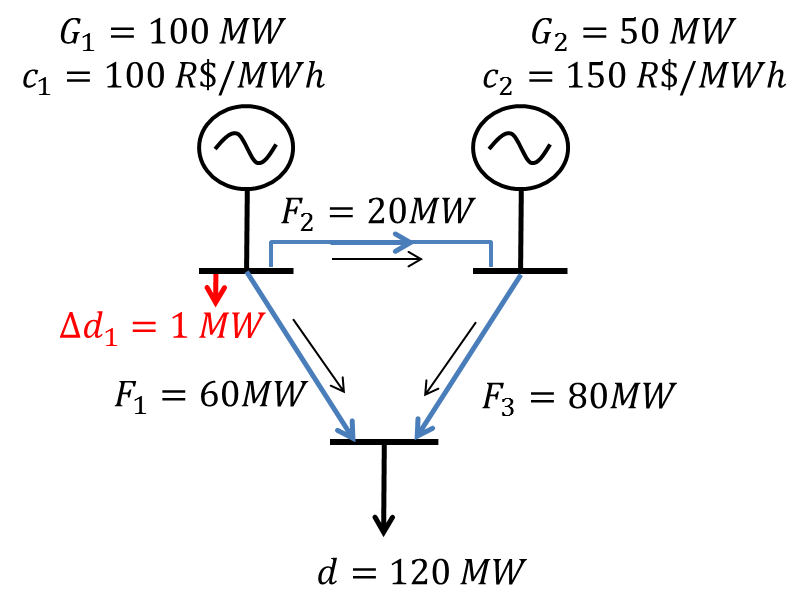
\includegraphics[scale=0.7]{aula4-18}\protect\caption{\label{fig:aula4-18} Aumento da demanda na barra 1 }
\end{centering}
\end{figure}
O custo adicional de operação encontrada é de $\pi_{1}=100$ R$\$$/MWh representado na figura (\ref{fig:aula4-19} ).
\begin{figure}[H]
\begin{centering}
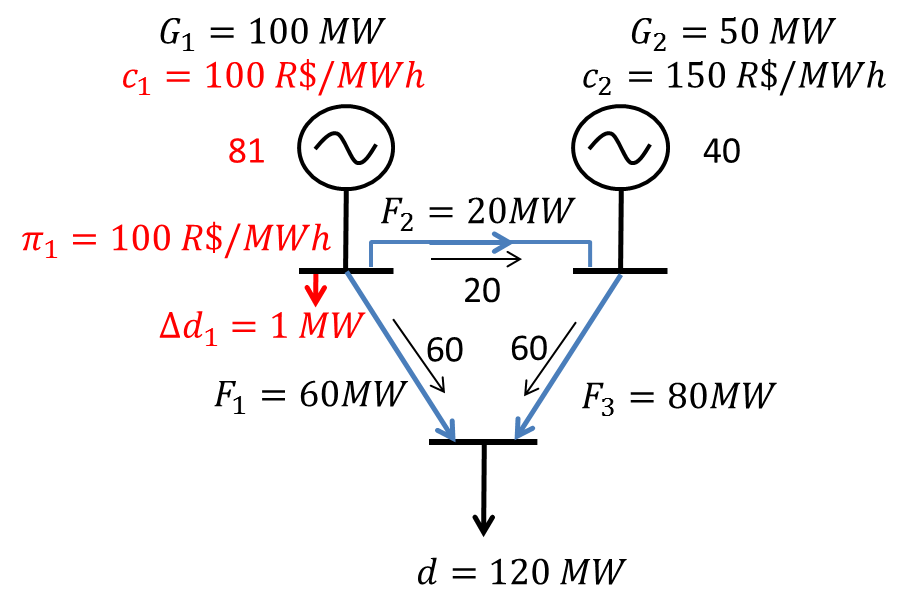
\includegraphics[scale=0.7]{aula4-19}\protect\caption{\label{fig:aula4-19} Custo adicional na barra 1 }
\end{centering}
\end{figure}

A barra $2$, o custo adicional de operação ótima para suprir $1$ MWh será representado na figura (\ref{fig:aula4-20} ) e a modelagem dada por:
\[
\min_{g_{i}\geq0,f_{l}}100g_{1}+150g_{2}
\]
\[
\begin{array}{ccccccc}
s.a:\\
g_{1} &  & -f_{1} & -f_{2} &  & = & 0\\
 & g_{2} &  & +f_{2} & -f_{3} & = & +1\\
 &  & f_{1} &  & +f_{3} & = & d\\
-60 & \leq & f_{1} &  &  & \leq & 60\\
-20 & \leq &  & f_{2} &  & \leq & 20\\
-80 & \leq &  &  & f_{3} & \leq & 80\\
g_{1} &  &  &  &  & \leq & 100\\
 & g_{2} &  &  &  & \leq & 50.
\end{array}
\]

\begin{figure}[H]
\begin{centering}
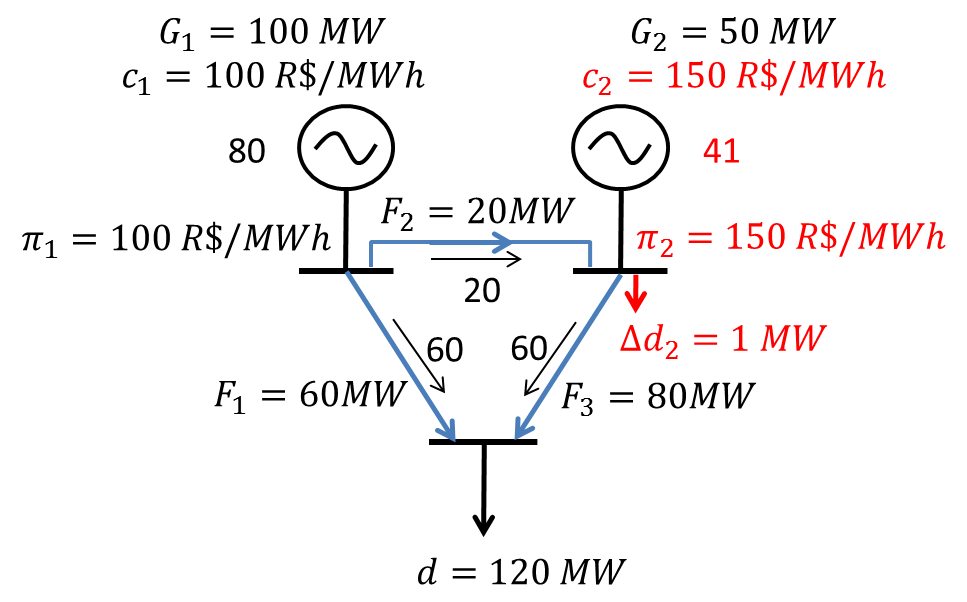
\includegraphics[scale=0.7]{aula4-20}\protect\caption{\label{fig:aula4-20} Custo adicional na barra 2}
\end{centering}
\end{figure}

Então,o custo adicional de operação encontrada é de  $\pi_{2}=150$ R$\$$/MWh.
Ao adicionar $1$ MWh na demanda, a barra $2$ irá atender essa demanda extra sem necessidade de cortar carga, conforme apresentado na figura (\ref{fig:aula4-21}).
\[
\min_{g_{i}\geq0,f_{l}}100g_{1}+150g_{2}
\]
\[
\begin{array}{ccccccc}
s.a:\\
g_{1} &  & -f_{1} & -f_{2} &  & = & 0\\
 & g_{2} &  & +f_{2} & -f_{3} & = & 0\\
 &  & f_{1} &  & +f_{3} & = & d+1\\
-60 & \leq & f_{1} &  &  & \leq & 60\\
-20 & \leq &  & f_{2} &  & \leq & 20\\
-80 & \leq &  &  & f_{3} & \leq & 80\\
g_{1} &  &  &  &  & \leq & 100\\
 & g_{2} &  &  &  & \leq & 50.
\end{array}
\]

\begin{figure}[H]
\begin{centering}
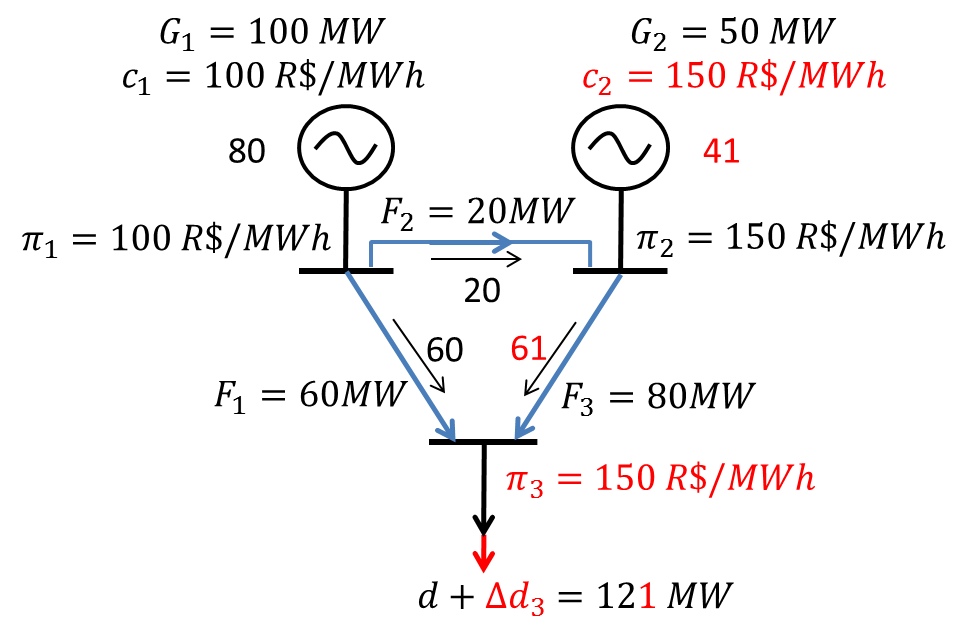
\includegraphics[scale=0.8]{aula4-21}\protect\caption{\label{fig:aula4-21} Custo adicional na demanda}
\end{centering}
\end{figure}

De maneira geral podemos associar os  $\pi_{i}$ que são as variáveis duais destas restrições do ponto ótimo do dual, da seguinte forma:
\[
\min_{g_{i}\geq0,f_{l}}100g_{1}+150g_{2}
\]
\[
\begin{array}{ccccccc}
s.a:\\
g_{1} &  & -f_{1} & -f_{2} &  & = & 0 (\pi_{1}) \\
 & g_{2} &  & +f_{2} & -f_{3} & = & 0 (\pi_{2})\\
 &  & f_{1} &  & +f_{3} & = & d (\pi_{3})\\
-60 & \leq & f_{1} &  &  & \leq & 60\\
-20 & \leq &  & f_{2} &  & \leq & 20\\
-80 & \leq &  &  & f_{3} & \leq & 80\\
g_{1} &  &  &  &  & \leq & 100\\
 & g_{2} &  &  &  & \leq & 50.
\end{array}
\]

Modelo DC linearizado

Este modelo adicionar mais uma restrição ao problema,sendo esta uma restrição linearizada do fluxo de potência visto na aula 3.
Para isso devemos incorporar a segunda lei de Kirchhoff:
\[
f_{l}=\frac{1}{x_{l}}(\theta_{ori(l)}-\theta_{des(l)}),
\]
o fluxo numa linha($f_{l}$) é proporcional ao inverso da reatância(${x_{l}$) e a diferença de ângulos entra as barras ($\theta_{ori(l)}-\theta_{des(l)}$). 
Supondo $x_{l}=1$:
$$f_{1}=\theta_{1}-\theta_{3}$$
$$f_{2}=\theta_{1}-\theta_{2}$$
$$f_{3}=\theta_{2}-\theta_{3}$$

Assim, temos uma restrição por ciclo:
$$f_{1}=\theta_{1}-\theta_{3}$$
$$f_{2}=\theta_{1}-\theta_{2}$$
$$f_{3}=\theta_{2}-\theta_{3}.$$

Criando assim uma dependência linear dos fluxos. Logo, $f_{1}-f_{2}=f_{3}$ ou $f_{2}=f_{1}-f_{3}$.
Devido a restrição acima e ao limite do fluxo na linha 2,temos: $-20\leq f_{1}-f_{3}\leq20$.

O despacho ótimo sem rede é inviável mesmo que exista capacidade suficiente
de transmissão.
Agora, supondo que amplie a capacidade de $f_{1}$ e pela dependência não
é viável este problema pelo fato de, $100-20=80$, que não atende a restrição de $-20\leq f_{1}-f_{3}\leq20$ (Figura \ref{fig:aula4-22}).

\begin{figure}[H]
\begin{centering}
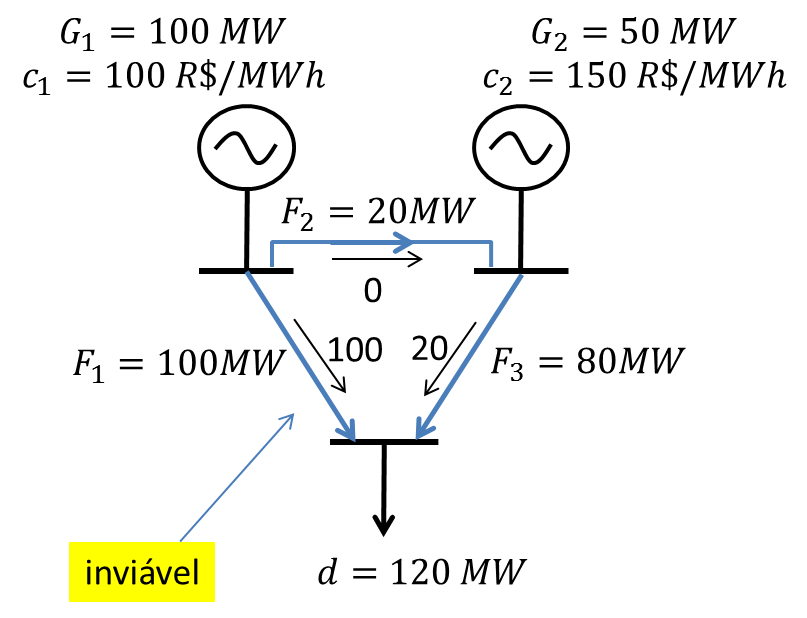
\includegraphics[scale=0.6]{aula4-22}\protect\caption{\label{fig:aula4-22} Problema inviável }
\end{centering}
\end{figure}

\subsection{Confiabilidade}
\begin{itemize}
\item Frequentes apagões demonstram que a confiabilidade do sistema ainda é um tema não resolvido, cortes de carga culminando em ações terríveis.
\item Os níveis de reserva (baixos) colocam o sistema em risco mesmo sob
contingências corriqueiras
\begin{figure}[H]
\begin{centering}
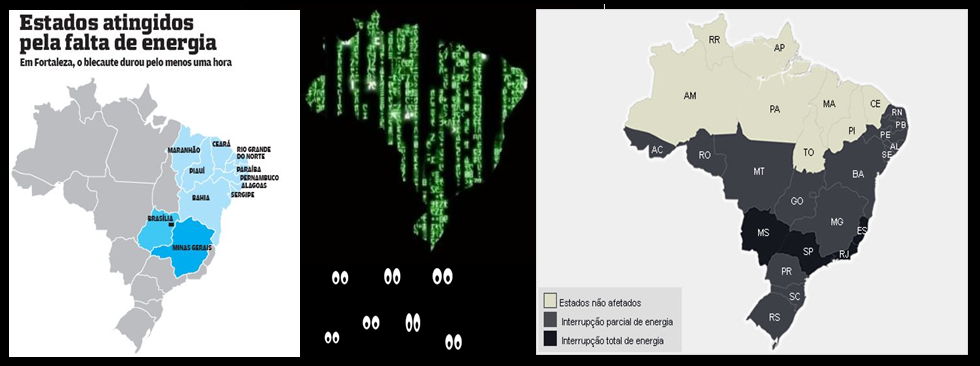
\includegraphics[scale=0.8]{aula4-23}\protect\caption{\label{fig:aula4-23} Apagões}
\end{centering}
\end{figure}
\item Falhas em cascata são uma das principais causas de grandes apagões
\item As redes elétricas são frequentes alvos de ataques
\begin{figure}[H]
\begin{centering}
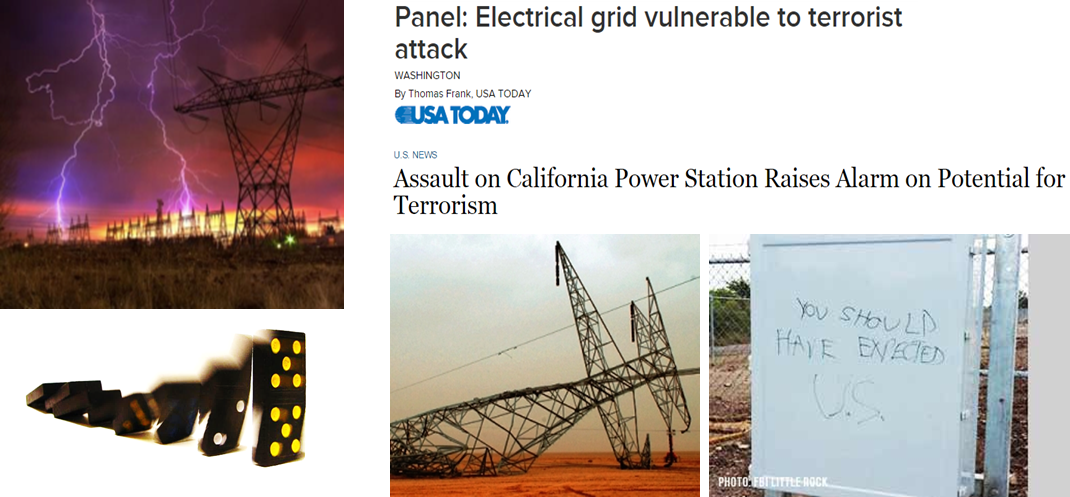
\includegraphics[scale=0.8]{aula4-24}\protect\caption{\label{fig:aula4-24} Falhas em cascata e ataques a redes elétricas }
\end{centering}
\end{figure}
\end{itemize}
Então é necessário garantir o suprimento da demanda com algum critério de "confiança", uma possibilidade para isso é associar a probabilidade à confiabilidade, conforme apresentado a seguir:

$$Prob(Demanda \, n\tilde{a}o \, suprida>0)\leq3\%$$,
ou seja, corte de carga ser positivo e limitado
.
Se a probabilidade de um dos geradores falhar é $5\%$ e as falhas
são independentes:

$P(Falhar\,G1)=P(Falha\,rG2)=5\%$

$P(Falhar\,G1\,e\,G2)=0,25\%$

Dado que os dois geradores são necessários para suprir a demanda.Logo, basta garantir que o sistema tenha reserva suficiente para suprir a demanda mesmo que um gerador falhe. Este é o critério $n-1$ de segurança. O sistema tem que atender a carga mesmo que um sistema da rede falhe.

Serviços ancillares são principais reservas girantes (capacidade ociosa nos geradores acoplados que permitem o sistema retomar o equilíbrio ,frequência e tensão, através do ``redespacho'' dos geradores remanescentes).

O modelo de despacho econômico de potência e reservas (Figura \ref{fig:aula4-25} tem como objetivo alocar as reservas de maneira que elas sejam entregaveis e garantem a entregabilidade das reservas mesmo que um gerador falhe. 

\begin{figure}[H]
\begin{centering}
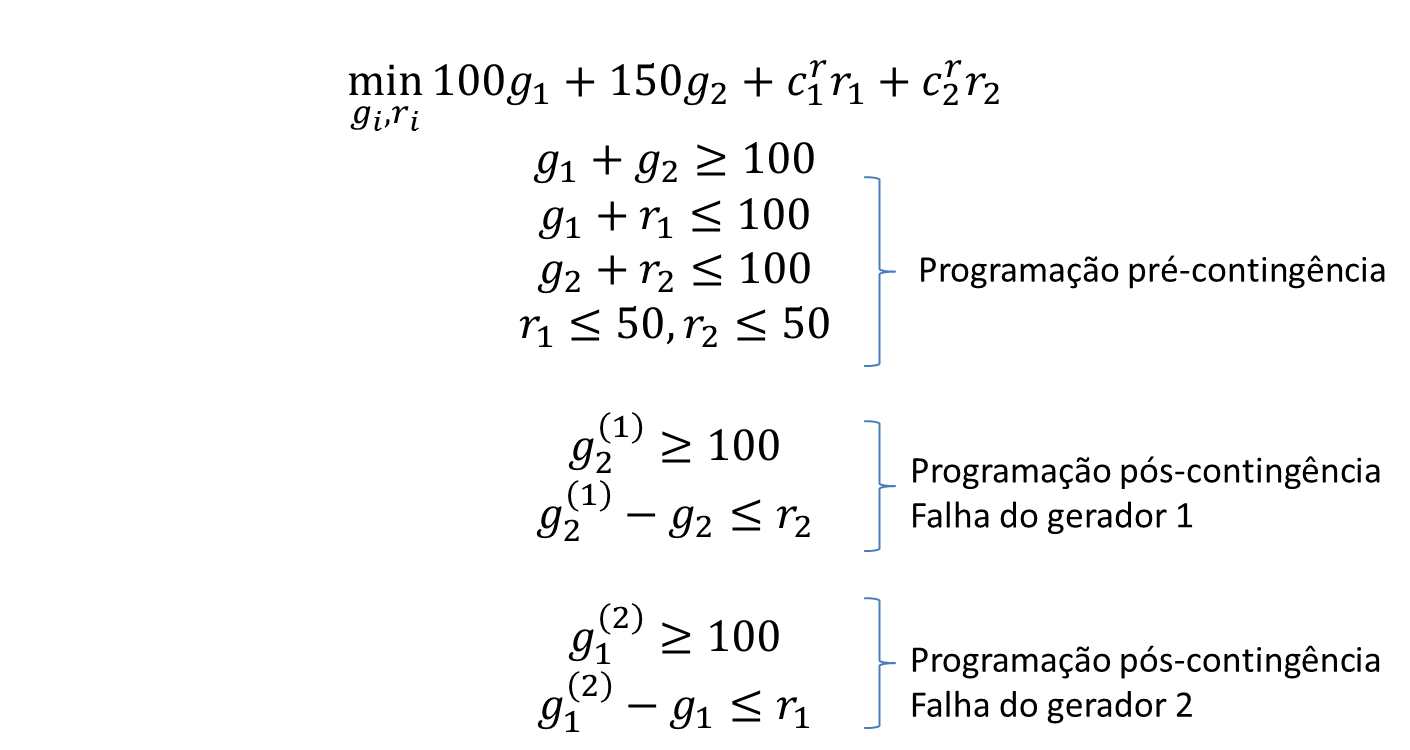
\includegraphics[scale=0.5]{aula4-25}\protect\caption{\label{fig:aula4-25} Modelo de despacho econômico de potência e reservas }
\end{centering}
\end{figure}

Programação pré-contingência ou programação nominal é a programação caso nada acontece ou seja,geração maior que a demanda, geração mais a reserva dentro da capacidade,geração mais a potencia de reserva com uma reserva máxima
da capacidade.

Caso ocorra falha do gerador $1$: redespacho inviável do gerador $2$ dentro da reserva programada de $50$ MW para atender a carga de $100$ Mw (Figura \ref{fig:aula4-26}).
\begin{figure}[H]
\begin{centering}
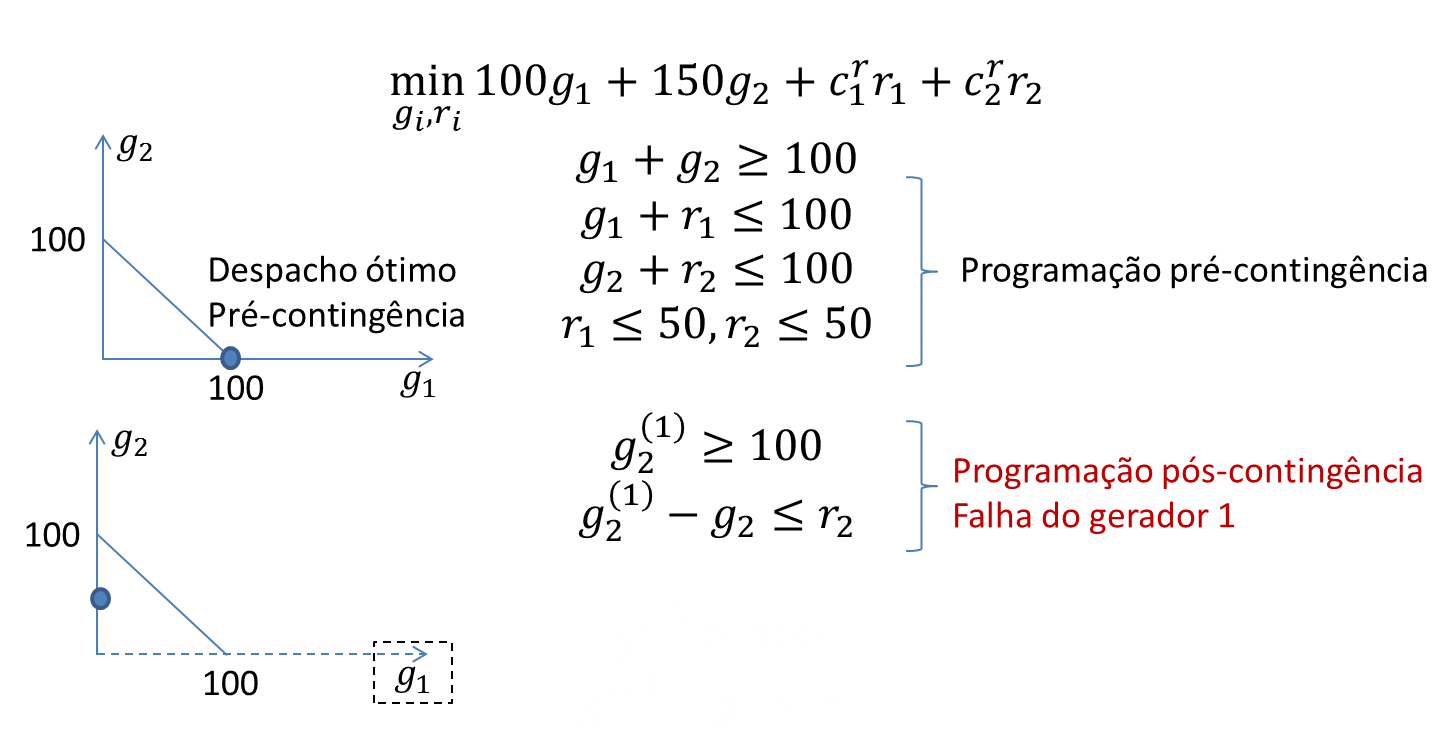
\includegraphics[scale=0.5]{aula4-26}\protect\caption{\label{fig:aula4-26} Falha do gerador 1}
\end{centering}
\end{figure}
Na figura \ref{fig:aula4-27} redespacho viável dentro das reservas programadas para atender a carga de $100$ Mw em qualquer estado pós-contingência. 

\begin{figure}[H]
\begin{centering}
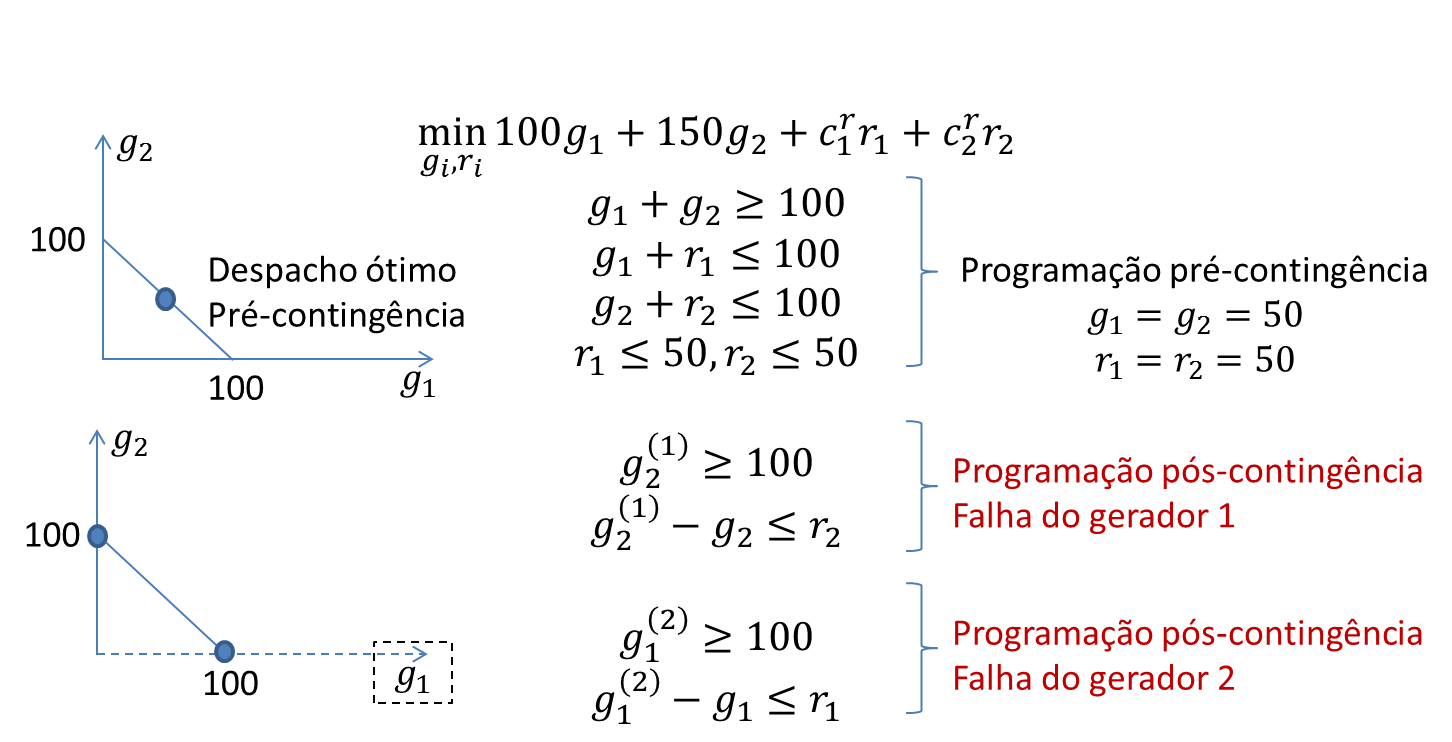
\includegraphics[scale=0.5]{aula4-27}\protect\caption{\label{fig:aula4-27} Falhar qualquer estado pós-contingência }
\end{centering}
\end{figure}

O despacho de potência e reservas apresentado de maneira geral pode ser expresso da seguinte maneira:
\begin{itemize}
\item Critério de confiabilidade n-K
\item Despacho de potência e reserva para o estado pré-contingência que garanta um redespacho viável mesmo que K elementos falhem
\item Garantir a entregabilidade das reservas
\item Considerando falaha de geradores e linhas de transmissão
\item Falha determinada pelo vetor de disponibilidade: vale 1 se o elemento está disponível e zero caso contrário.
\item $$a(k)=\left[a^{G}(k)|a^{L}(k)\right]\in\{0,1\}^{n}$$
\item $$\sum_{i\in U}a_{i}^{G}(k)+\sum_{l\in L}a_{l}^{L}(k)\geq n-K$$
\end{itemize}
Assim temos a modelagem completa :
\begin{figure}[H]
\begin{centering}
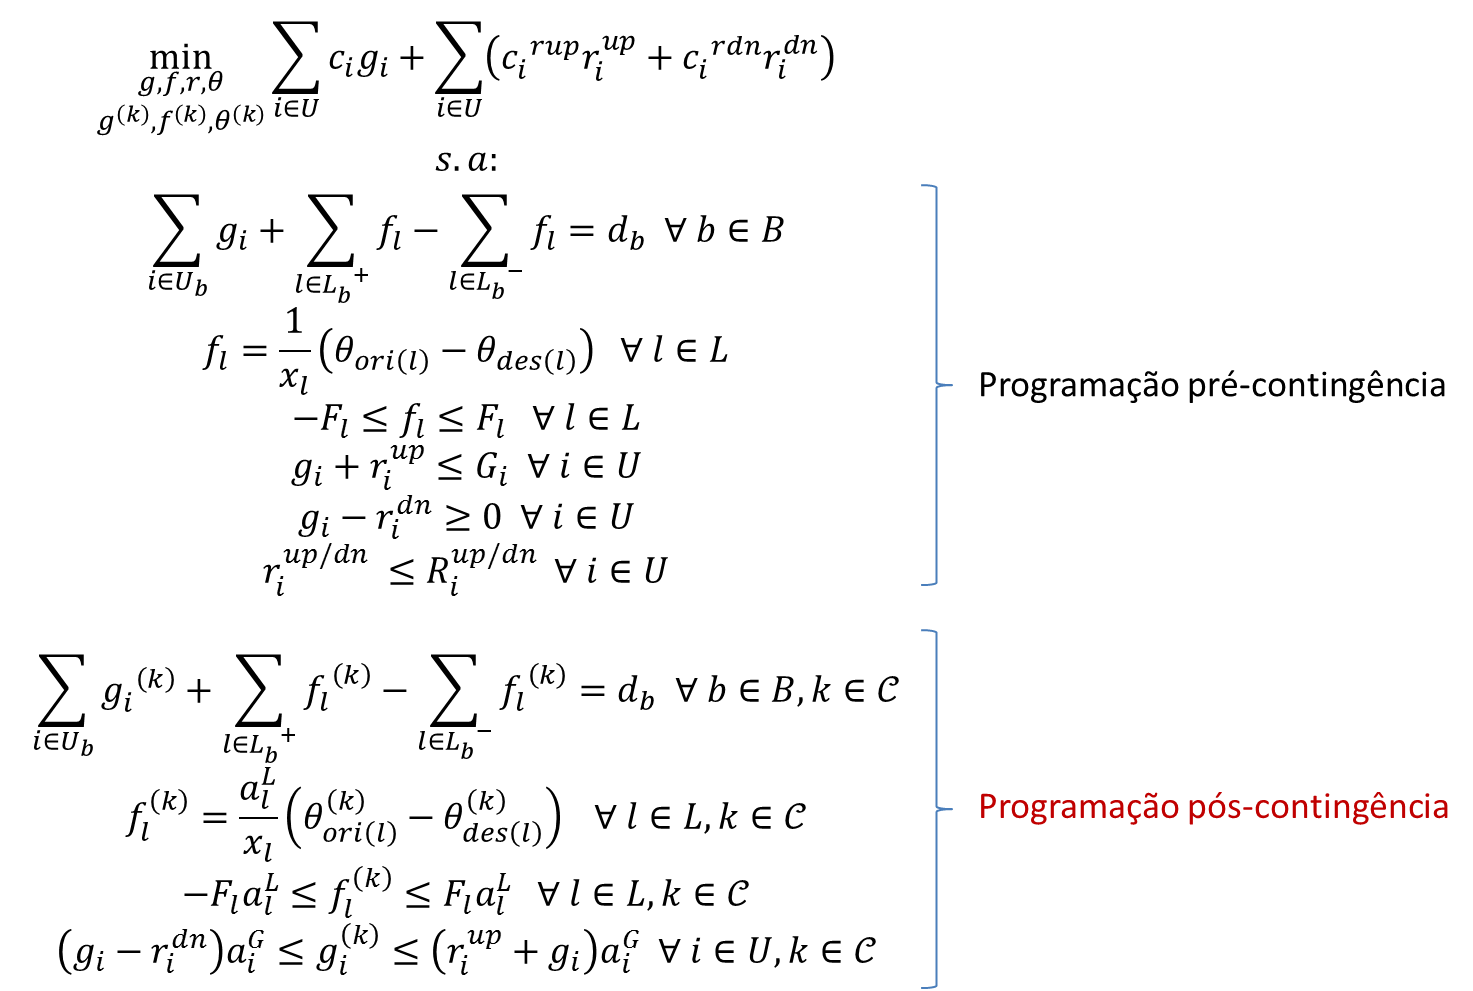
\includegraphics[scale=0.5]{aula4-28}\protect\caption{\label{fig:aula4-28} Problema completo}
\end{centering}
\end{figure}
Considerando todo cenário de demanda líquida:
\begin{figure}[H]
\begin{centering}
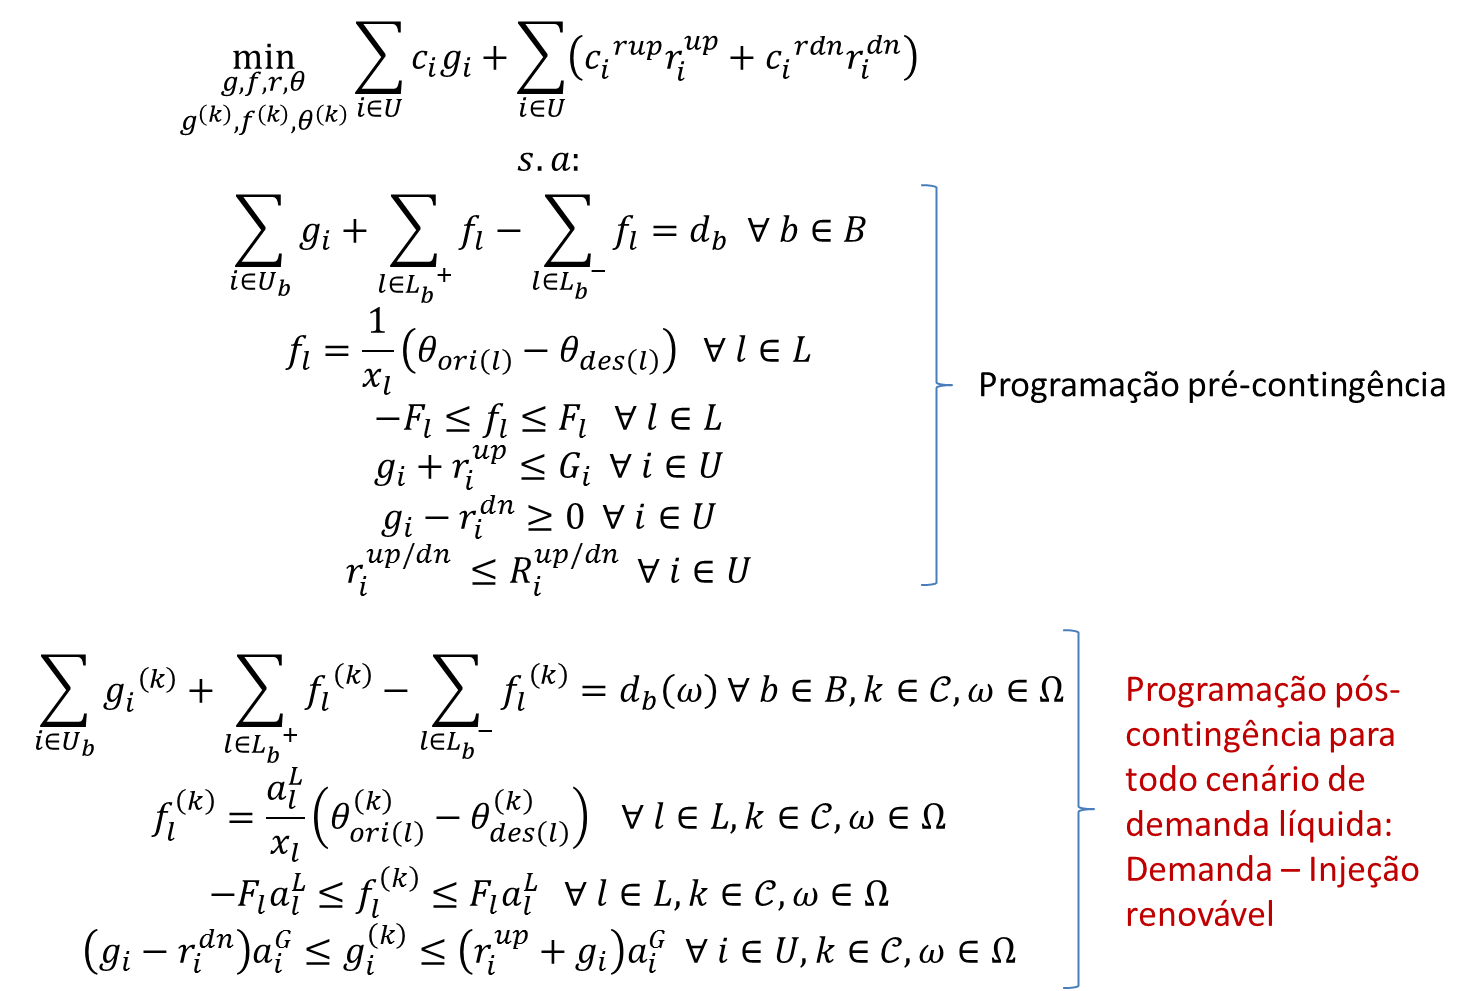
\includegraphics[scale=0.5]{aula4-29}\protect\caption{\label{fig:aula4-29} Problema completo considerando todo cenário de demanda líquida}
\end{centering}
\end{figure}

\textbf{Preço da energia com segurança}
\begin{itemize}
\item O preço da energia está associado ao incremento de custo devido a
um incremento na demada dado por:

\[
\pi_{b}=\pi_{b}^{pre}+\sum_{k\in C}\pi_{bk}^{pos}\forall b\in B
\]
Onde $\pi_{b}^{pre}$ e $\pi_{bk}^{pos}$ são as variáveis duais das
restrições abaixo:

\[
\sum_{i\in U_{b}}g_{i}+\sum_{l\in L_{b}^{+}}f_{l}-\sum_{l\in L_{b}^{-}}f_{l}=d_{b}(\pi_{b}^{pre})\forall b\in B
\]


\[
\sum_{i\in U_{b}}g_{i}^{(k)}+\sum_{l\in L_{b}^{+}}f_{l}^{(k)}-\sum_{l\in L_{b}^{-}}f_{l}^{(k)}=d_{b}(\pi_{b}^{pos})\forall b\in B,k\in C
\]

\end{itemize}

\subsection{Unit Commitment}
\begin{itemize}
\item $v_{it}\in\{0,1\}$: vale $1$ se o gerador $i$ estiver ligado em $t$
\item Adicionar o custo de start-up e shutdown $C^{on}x_{it}^{on}+C^{off}x_{it}^{off}$
\item \[
v_{it}-v_{it-1}=x_{it}^{on}-x_{it}^{off}=1-0
\]


Restrições de rampa:

\[
-\Delta_{i}^{dn}\leq g_{it+1}-g_{it}\leq\Delta_{i}^{up}
\]
\begin{figure}[H]
\begin{centering}
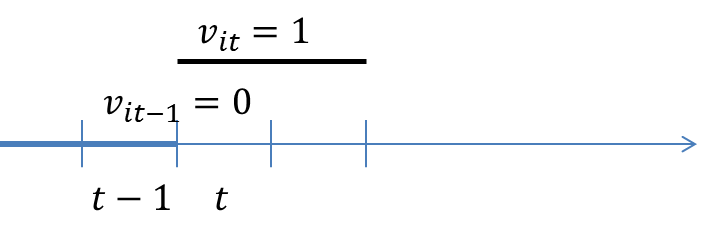
\includegraphics[scale=0.5]{aula4-30}\protect\caption{\label{fig:aula4-30} }
\end{centering}
\end{figure}

\item \[
v_{it}-v_{it-1}=x_{it}^{on}-x_{it}^{off}=0-1
\]


\begin{figure}[H]
\begin{centering}
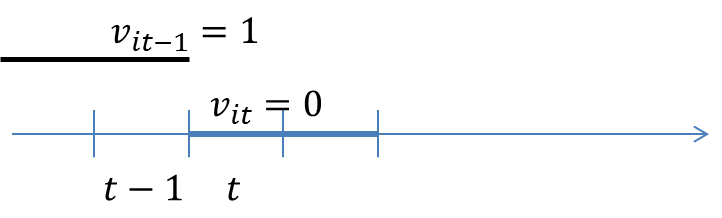
\includegraphics[scale=0.5]{aula4-31}\protect\caption{\label{fig:aula4-31} }
\end{centering}
\end{figure}
\end{itemize}
\subsection{Operacionalização}

Planejamento para o dia seguinte

\begin{itemize}
\item Modelos de unit commitment: custo varáveis e fixos de partida, desligamento,restrições de tecnologias, restrições de rede e confiabilidade (segurança).
\item Definir quais centrais estarão ligadas, em quais horas e suas quantidades de produção nominal e reservas.
\item Incertezas: demanda, geração renovável, disponibilidade de equipamentos
\end{itemize}

\begin{figure}[H]
\begin{centering}
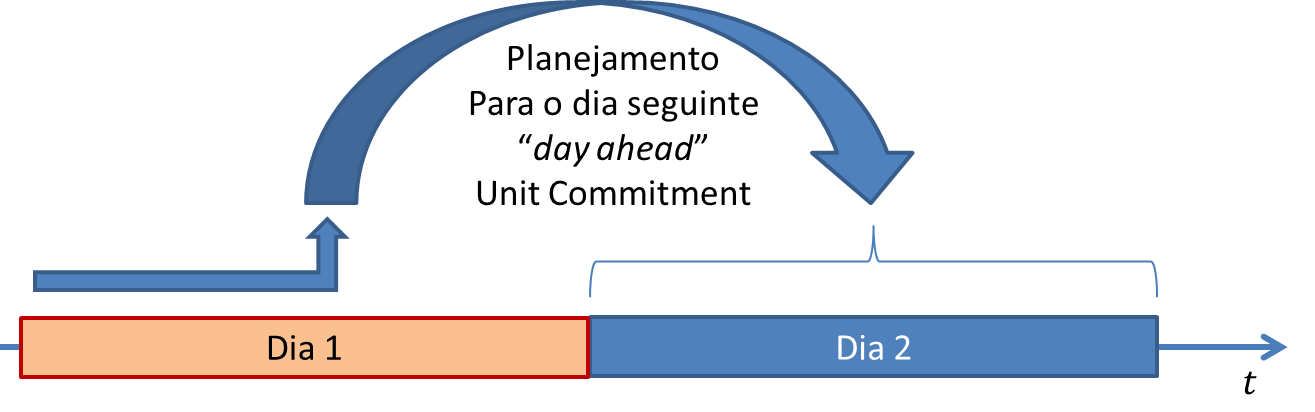
\includegraphics[scale=0.5]{aula4-32}\protect\caption{\label{fig:aula4-32} Planejamento para o dia seguinte }
\end{centering}
\end{figure}

Operação em tempo real
\begin{itemize}
\item Modelos de despacho econômico: custos variáveis, restrições tecnologias,
restrições de rede mais detalhadas e confiabilidade (segurança).
\item Definir quantidades de produção para os próximos 5 minutos
\item Principal incerteza: disponibilidade de equipamentos, injeção intermitente (renováveis)
\end{itemize}
\begin{figure}[H]
\begin{centering}
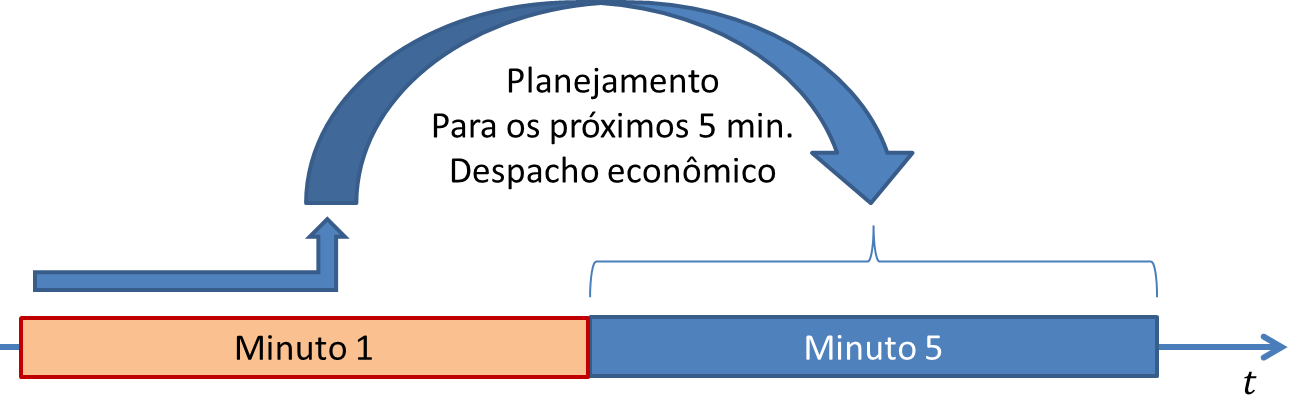
\includegraphics[scale=0.5]{aula4-33}\protect\caption{\label{fig:aula4-33} Operação em tempo real}
\end{centering}
\end{figure}